%%% LaTeX Template: Two column article
%%%
%%% Source: http://www.howtotex.com/
%%% Feel free to distribute this template, but please keep to referal to http://www.howtotex.com/ here.
%%% Date: February 2011

%%% Preamble
\documentclass[	DIV=calc,%
							paper=a4,%
							fontsize=11pt,%
							twocolumn]{scrartcl}	 					% KOMA-article class

\usepackage{lipsum}													% Package to create dummy text

\usepackage[english]{babel}										% English language/hyphenation
\usepackage[protrusion=true,expansion=true]{microtype}				% Better typography
\usepackage{amsmath,amsfonts,amsthm}					% Math packages
\usepackage[pdftex]{graphicx}									% Enable pdflatex
\usepackage[svgnames]{xcolor}									% Enabling colors by their 'svgnames'
\usepackage[hang, small,labelfont=bf,up,textfont=it,up]{caption}	% Custom captions under/above floats
\usepackage{epstopdf}												% Converts .eps to .pdf
\usepackage{subfig}													% Subfigures
\usepackage{booktabs}												% Nicer tables
\usepackage{fix-cm}													% Custom fontsizes



%%% Custom sectioning (sectsty package)
\usepackage{sectsty}													% Custom sectioning (see below)
\allsectionsfont{%															% Change font of al section commands
	\usefont{OT1}{phv}{b}{n}%										% bch-b-n: CharterBT-Bold font
	}

\sectionfont{%																% Change font of \section command
	\usefont{OT1}{phv}{b}{n}%										% bch-b-n: CharterBT-Bold font
	}


\definecolor{brsugrey}{rgb}{0.9, 0.9, 0.9}
\definecolor{brsublue}{rgb}{0, 0.594, 0.949}


\newcommand{\upperRomannumeral}[1]{\uppercase\expandafter{\romannumeral#1}}

%%% Headers and footers
\usepackage{fancyhdr}												% Needed to define custom headers/footers
	\pagestyle{fancy}														% Enabling the custom headers/footers
\usepackage{lastpage}	

% Header (empty)
\lhead{}
\chead{}
\rhead{}
% Footer (you may change this to your own needs)
\lfoot{\footnotesize \texttt{P\&S} \textbullet ~ Moriarty, Hagg \textbullet ~ Planning and Scheduling Summary}
\cfoot{}
\rfoot{\footnotesize page \thepage\ of \pageref{LastPage}}	% "Page 1 of 2"
\renewcommand{\headrulewidth}{0.0pt}
\renewcommand{\footrulewidth}{0.4pt}



%%% Creating an initial of the very first character of the content
\usepackage{lettrine}
\newcommand{\initial}[1]{%
     \lettrine[lines=3,lhang=0.3,nindent=0em]{
     				\color{brsublue}
     				{\textsf{#1}}}{}}

%%% Title, author and date metadata
\usepackage{titling}															% For custom titles

\newcommand{\HorRule}{\color{brsublue}%			% Creating a horizontal rule
									  	\rule{\linewidth}{1pt}%
										}

\pretitle{\vspace{-30pt} \begin{flushleft} \HorRule 
				\fontsize{25}{25} \usefont{OT1}{phv}{b}{n} \color{gray} \selectfont 
				}
\title{Planning and Scheduling\\ Summary}	% Title of your article goes here
\posttitle{\par\end{flushleft}\vskip 0.5em}

\preauthor{\begin{flushleft}
					\large \lineskip 0.25em \usefont{OT1}{phv}{b}{sl} \color{brsublue}}
\author{Alexander Moriarty, Alexander Hagg, }									% Author name goes here
\postauthor{\footnotesize \usefont{OT1}{phv}{m}{sl} \color{Black} 
					BRS University of Applied Sciences 		% Institution of author
					\\ Planning and Scheduling summary
					\par\end{flushleft}\HorRule}

\date{\today}							% No date



%%% Begin document
\begin{document}
\maketitle
\thispagestyle{fancy} 			% Enabling the custom headers/footers for the first page 
% The first character should be within \initial{}
\initial{P}\textbf{lanning and Scheduling mid semester summary in preparation of exam}

\section{Introduction}
\begin{itemize}
 \item Conceptual model
  \begin{figure}[h]
    \centering
    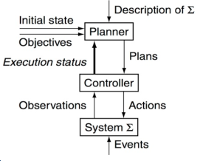
\includegraphics{./img/conceptual_model.png}
    \caption{Conceptual model}
  \end{figure}
 
 \item State-transition system
 
	$\Sigma = (S,A,E,\gamma)$
  \begin{itemize}
   \item $S$: states
   \item $A$: actions
   \item $E$: events
   \item $\gamma$: state-transition function
  \end{itemize} 	

 \item Objectives
 \begin{itemize}
  \item $S_g$: set of goal states
  \item utility function
 \end{itemize}
 
 \item Restrictive assumptions
 \begin{itemize}
  \item A0: finite $\sigma$
  \item A1: $\sigma$ is fully observable (observation function is id() )
  \item A2: deterministic $\sigma$, action: one possible outcome
  \item A3: static $\sigma$: E is empty
  \item A4: attainment goals: goal state or a set of goal states
  \item A5: sequential plans
  \item A6: implicit time (instant transitions)
  \item A7: off-line planning
 \end{itemize}
 
 \item Classical planning
 \begin{itemize}
  \item requires all eight restrictive assumptions
  \item Given $(\Sigma, s_0, S_g)$
  \item find a sequence of actions $<a_1,a_2,...,a_n>$
  \item that produces sequence of transitions $s_1 = \gamma(s_0,a_1), ...$
  \item such that $s_n \in S_g$
 \end{itemize}
 
 \item Relaxing assumptions
 \emph{Is this necessary?} 
 
\end{itemize}



\section{Search and Complexity}
\subsection*{Problem Solving Agents}
\begin{itemize}
\item
\end{itemize}

\subsection*{Problem Types}
\begin{itemize}
\item Deterministic, fully observable
\item Non-observable
\item Nondetermin
\end{itemize}
\subsection*{Problem Formulation}
\subsection*{Example Problems}
\subsection*{Basic Search Algorithms}

\section{Logic and Inference}
\input{sections/logic_and_inference}

\section{Representing Plans}
\begin{itemize}
\item \textbf{Classical representation}

	\begin{itemize}
	\item function-free FOL
	\item Atom: predicate symbol and args $on(c1,c3)$, $on(c1,x)$
	\item Ground expression: instantiated var $on(c1,c3)$
	\item Nonground expression: at least one var $on(c1,x)$
	\item Substitution $\theta = {x_1 \leftarrow v_1, ... }$ 
	\item Instance of expression e: result of applying $\theta$ 
	\end{itemize}
\item State : set of ground atoms

\item Operator
	\begin{itemize}
	\item (name, precond, effects)
	\item $take(k,l,c,d,p) \\ precond: belong(k,l) \\ effects: holding(k,c), \neg empty(k) $
	\end{itemize}
	
\item Action
	\begin{itemize}
	\item ground instance of operator
	\end{itemize}
	
\item Notation
	\begin{itemize}
	\item $S^+$, $S^-$, $precond^+$, ...
	\end{itemize}

\item Result of action
	\begin{itemize}
	\item $\gamma (s,a) = ( s \backslash effects^-(a) \cup effects^+(a)$
	\end{itemize}

\item Planning problem
	\begin{itemize}
	\item given: domain (L, O) (Language, Operators)
	\item $P = (\Sigma,s_0,S_g)$ (state-trans., initState, goal formula)
	\item $\Sigma = (S,A,E,\gamma)$
	\end{itemize}

\item Plan
	\begin{itemize}
	\item $\sigma = \langle a_1,a_2,...,a_n \rangle$
	\item is a solution for P if it is executable and achieves g
	\end{itemize}
	
\end{itemize}

\begin{itemize}
\item \textbf{Set-theoretic representation}

	\begin{itemize}
	\item classical representation + restriction to PL
	\item collection of propositions (bool) instead of ground atoms
	\item effects: delete, add
	\end{itemize}
\item exponential blow-up		
\end{itemize}

\begin{itemize}
\item \textbf{State-Variable representation}

	\begin{itemize}
	\item State variables: pos(x) = y (if block x is on block y)
	\end{itemize}
\end{itemize}

\begin{itemize}
\item \textbf{Expressive power}
\item linear time/space conversion between all three representations, except for expBlowup on conversion to set-theoretic
	\begin{itemize}
	\item classical rep: most popular
	\item set-theoretic: much more space, useful for algorithms that manipulate ground atoms directly
	\item state-variabl: equivalent to classical, more natural for engineers, used for non-classical planning problems (incl. functions!) 	
	\end{itemize}
\end{itemize}

\section{Complexity of Classical Planning}
\begin{itemize}
\item \textbf{Complexity analysis}
\item general idea: translate classical planning -> language-recognition problem and examine its complexity
\item Language L, alphabet A
\item recognition procedure R(x): yes iff $x \in L$, else no or fail to terminate

	\begin{itemize}
	\item \textbf{Plan-Existence} P
	\item Problem has solution
	\item \textbf{Plan-Length} (P,n)
	\item Problem has solution <= n
	\end{itemize}

\item Runtime, space complexity

\item \textbf{Restrictions of classical planning}
\begin{itemize}
	\item Operators are fixed or input?
	\item Allow infinite initial states?*	
	\item Allow function symbols?*
	\item Allow negative effects?
	\item Allow neg. preconditions?
	\item Allow >1 preconditions?
	\item Operators have conditional effects?*
\end{itemize}

\item *: outside CP

\item \textbf{(Un)decidability}

\begin{tabular}{|c|c|c|}
\hline 
& \multicolumn{2}{c|}{Decidability} \\ 
\hline 
function symbols & Plan-Existence &Plan-Length \\ 
\hline 
no (CP) & dec & dec \\ 
\hline 
yes & semidec & dec \\ 
\hline 
\end{tabular} 


\item \textbf{Complexity results}
\item Well I guess, Plan-Existence is less complex than Plan-Length (AM?)

\item \textbf{Equivalences}
\item Set-theoretic and classical are basically identical
\item Both: exponential blowup (input)
\item Class. and state-var are basically equivalent 
\item (state-var:some restrictions not possible)

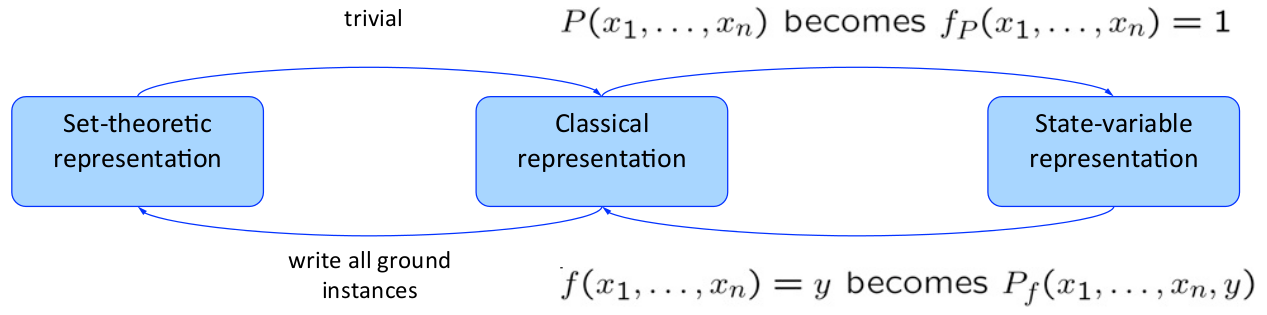
\includegraphics[width=0.48\textwidth]{./img/conversions.png}

\end{itemize}

\section{State Space Planning}
\begin{itemize}
\item \textbf{State space vs plan space}
\item State space
	\begin{itemize}
	\item Node: state of the world
	\item Plan: path through space
	\end{itemize}
	
\item Plan space
	\begin{itemize}
	\item State: set of partially instantiated operators and some constraints
	\item Impose more constraints until Plan
	\end{itemize}

\item \textbf{Linear search}
\item Work on one goal until completely solved
\item Order of problem solving is linearly-related to order in which plan actions are executed
\item Maintain \textbf{goal stack}
\item Implications
	\begin{itemize}
	\item No interleaving of goal achievement
	\item Efficient search if goals do "not" interact
	\end{itemize}
	
\item \textbf{Means-End analysis}
\item Search relevant aspects of problem, means/operators, ends/goals
	\begin{itemize}
	\item Start from the goal
	\item find difference to start state
	\item find operator that reduces this difference
	\end{itemize}
\item General Problem Solver (GPS)
	
\item \textbf{Forward search}
\\
$s \leftarrow s_0$\\
$\pi \leftarrow empty\_plan$\\
$loop$\\
if s satisfies g $\rightarrow$ return $\pi$\\
$E \leftarrow \{$a ground instance of o $\in$ O, precond(a) true in s\}\\
if $E=\emptyset \rightarrow$ failure\\
nondet choose a $\in$ E\\
$s \leftarrow \gamma(s,a)$\\
$\pi \leftarrow \pi,a$\\
$endloop$
\item = sound,complete
\item breadth-first, best-first
	\begin{itemize}
	\item sound and complete
	\item memory exponential in length of solution
	\end{itemize}
\item depth-first, greedy search
	\begin{itemize}
	\item Worst-case mem is linear in length of solution
	\item Sound, but not complete 
	\item but CP has only finite states $\rightarrow$ loop-checking solves completeness
	\end{itemize}	
\item large branching factor (need good heuristic / pruning)

\item \textbf{Backward search}
\item Means-end analysis
\item start at goal and compute inverse state transitions 
\item a makes at least one of g's literals true and non false
\item $g' = \gamma^{-1}(g,a) = (g\backslash effects(a)) \cup precond(a)$
\\
$\pi \leftarrow empty\_plan$\\
$loop$\\
if s satisfies g $\rightarrow$ return $\pi$\\
$A \leftarrow \{ a|a$ ground instance of o in O and $g' = \gamma^{-1}(g,a)$ defined $\}$\\
if $A=\emptyset$ failure \\
nondet choose $a \in A$ \\
$\pi \leftarrow a,\pi$ \\
$g \leftarrow \gamma^{-1}(g,a)$ \\
$endloop$
\item Branching factor smaller, but can be big because of more actions than needed

\item \textbf{Lifting}
\item reduce branching factor by \textbf{partially instantiating} operators (=lifting)


\item \textbf{STRIPS}
\item STRIPS assumption -> solved frame problem
\item difference
\item sub-goals
\item applicability
\item plan execution and learning

\item \textbf{Block stacking}

%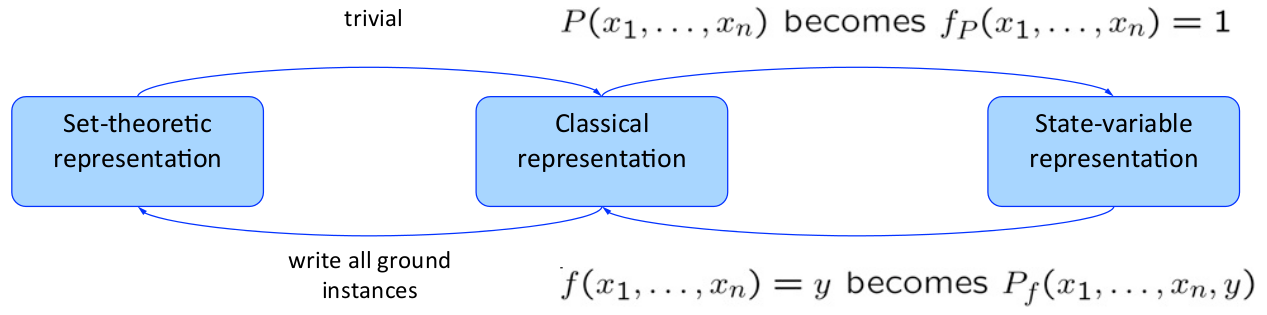
\includegraphics[width=0.48\textwidth]{./img/conversions.png}

\end{itemize}

\section{Plan Space Planning}
\begin{itemize}
\item \textbf{Motivation}
\item in SSP: try all orderings before "no solution"
\item PSP: do not commit to orderings, instantiations, etc.

\item \textbf{Partial Order Plan vs Total Order Plan}
\item POP: "parallel" paths

\item \textbf{PSP}: Backward search from g
\item Each node is \textbf{partial plan}
	\begin{itemize}
	\item \{ part.-instantiated operators (\textbf{steps}) \}
	\item Sets of constraints
	\end{itemize}
\item Refine until solution

\item \textbf{Constraints}
	\begin{itemize}
	\item \textbf{Precedence constraints}: a must precede b
	\item \textbf{Binding constraints}: (in)equality
	\item \textbf{Causal links}: use step a to establish prec p needed by c
	\end{itemize}
\item No more \textbf{flaws} $\rightarrow$ plan

\item \textbf{Representation}
\item P = $\langle$ steps, orderings, bindings, causallinks $\rangle$

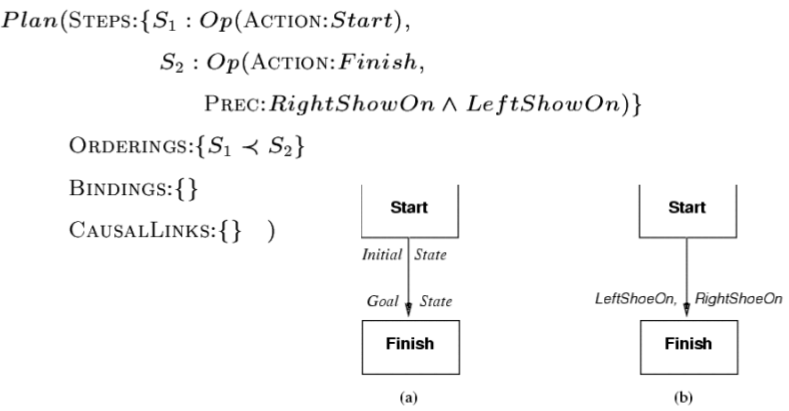
\includegraphics[width=0.48\textwidth]{./img/psp_representation.png}

\end{itemize}

\section{Graph Based Planning}
\input{sections/graph_based_planning}

\section{Satisfiability Based Planning}
\input{sections/satisfiability_based_planning}

\section{Hierarchical Task Network Planning}

* partial ordering enables interleaving of tasks. E.g. we need a hammer and a drill and we do not care in what order


\end{document}